\documentclass{sig-alternate}

\title{CS 472 --- Project 3}
\subtitle {GAs \& DEs --- A Land of Lisp Approach}

\numberofauthors{1}

\author{
\alignauthor
Steven White \\
  \email{swhite24@mix.wvu.edu}\\
  8258
}

\begin{document}
\date{22 March 2012}
\pagenumbering{arabic}

\maketitle
\section{abstract}
Test drive abstract. More to come.  Need to list all subsequent
sections along with a brief summary.

\section{Introduction}
Land of lisp did rats.  I do rats with de \& ga.

\section{Models}
Description of \emph{Land of Lisp} rat model here.

\begin{figure}
\centering
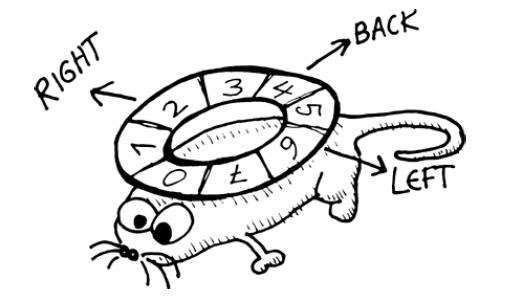
\includegraphics[width=0.4\textwidth]{rat_wheel.PNG}
\caption{Gene ``wheel'' depicting directions of rat travel.}
\end{figure}

\section{Algorithms}
Compare and constrast DE with GA.  Some pseudo-code.

\subsection{Genetic Algorithms}
GA specific alg info here.

\subsection{Differential Evolution}
DE specific alg info here. Only using DEMO/parent at this point.

\subsection{Comparison}
Compare \& contrast GA with DE.

\section{Expectations}
List of research questions (RQ1, RQ2, etc) and/or hypotheses
(H1, H2, etc).  Must include two-population hypothesis.

\section{Results}
Performance, effectiveness, better on one or multiple
objectives.  Graphs, etc.

\section{Validity}
Comment on limitations of study.

\section{Conclusion}
Return to section \emph{Expectations} and address whether the results
match what was expected.

\section{Further Work}
Discuss paths not taken.  What would be next step?

\section{References}
Self-explanatory.

\section{Listings}
All source code and example output.  Divide code into three files
--- de.lisp, ga.lisp, and gade.lisp.

\end{document}
